\documentclass{internal-report}
\usepackage[UTF8]{ctex}
\usepackage{booktabs}
\usepackage{multirow}
\usepackage{amsmath,amssymb}

% STATUS: done
% LAST_MODIFIED: 2026-08-08

\title{S3 内部报告：储能协同优化}
\author{MathModel 建模小组}
\date{2026-08-08}

\begin{document}

\maketitle

\section{子问题概述}

问题三（S3）要求在给定任务调度与逐时负荷的基础上，建立储能协同优化模型，
设计储能充放电策略，并分析储能系统对\textbf{运行成本、碳排放、区域峰值净购电功率
和负荷波动程度}四项指标的影响。官方口径（说明 4）：以
$Baseline\_AI\_IT\_Load + NonAI\_IT\_Load$ 为给定 IT 负荷（设施负荷 $=$ IT$\times$PUE，
数据列 $Total\_Load$ 已折算），仅优化储能充放电、购售电及新能源分配，不优化任务调度。

经阶段 1 方案探索与 2.1 实证（人类裁定），最终口径为：
\textbf{储能协同优化线性规划（LP），成本目标 + 碳排 $\varepsilon{=}1.00$ 约束，
受限消纳主口径（B1）}。$\varepsilon$ 三档（0.90/0.95/1.00）经全档核验
$\varepsilon<1.00$ 全部区域不可行（碳排已近可行下限），故以 $\varepsilon=1.00$
为唯一主解，碳排作为评价指标报告（D4 修订，决策日志 2.1）。

\section{数据与预处理}

数据源：$region\_time\_data$（0--2406h $\times$ 6 区逐时电价/碳强度/负荷/新能源/储能基准）、
$storage\_information$（储能参数）、$GPU\_information$（PUE，核验用）。
阶段 1.4 预处理产出 \texttt{outputs/data/s3-preprocessed.pkl}（面板：电价/卖电价/碳强度/
设施负荷/可用新能源 + 储能参数 + 碳基准 + 自检）。

关键数据事实（A 类验证，\texttt{verify-sub3-20260808.md}）：
设施负荷 $Total\_Load = IT\times PUE$ 精确成立；新能源可用序列六区域同分布
（均值 800、min 500、max 1100 MW）；基准弃电率 79.2\%；基准轨迹 D/E/F 违反
$SOC(2406)\ge Initial$ 硬约束（不可作公平对照）；D/E/F 卖电 2400h 全覆盖
（SellPrice$\le$Price 恒成立，无购电$\to$卖电套利窗口）。

\textbf{受限消纳假设（B1 裁定，阶段 3.1 论证修订）}：新能源消纳能力（直供+充电）
逐时锚定基准观测值 $R_t+C^r_t \le UsedRenewable_t+RenewableCharge_t$。
\textbf{口径性质声明}：该上限为\textbf{消纳能力假设}——基于基准轨迹的观测值
（基准弃电率 79.2\% 反映其运行策略，而非电网物理能力的直接测量）。选此口径的
工程依据：(i) 电网消纳能力受线路/调峰物理约束，现实中存在逐时上限；
(ii) 以基准观测值作为该上限的保守估计，避免无依据地放大消纳能力。
\textbf{敏感性声明}：自由消纳口径（$R_t+C^r_t\le Avail_t$）下，可用新能源恒大于
负荷（均值 800 vs 峰值 652 MW），最优解购电 $\approx 0$、成本趋近理想下界
（F1 口径 b）——该结果在物理上成立但脱离"消纳能力有限"的工程现实；
两口径结果均报告（主口径受限 + 敏感性自由），论文以受限口径为主。

\section{模型}

完整推导见 \texttt{solution/model-notes/math-sub3.tex}。主时域 $0$--$2399$ 为评价窗口，
$2400$--$2405$ 结清段仍计入成本结算，$2406$ 仅状态结算（$E_{2406}=E_{2405}$）。
\textbf{结清段碳帽说明（阶段 3.1 补充）}：碳 $\varepsilon$ 约束仅限主时域（C7），
结清段购电只计成本不设碳帽——若结清段出现"低价高碳"时段组合，LP 有动机将购电
挪至结清段规避碳帽。本数据中结清段购电极少（基准 A/B/C 无购电、D/E/F 净购电为负，
H6 佐证），但未做电价平移敏感性检验，属局限声明。

\subsection{决策变量（每区域 $r$，$t=0,\ldots,2405$）}

$G_t$ 购电、$S_t$ 卖电、$R_t$ 新能源直供、$C^g_t$ 电网充电、$C^r_t$ 新能源充电、
$D_t$ 放电（均 $\ge0$）、$E_t$ SOC（时段末，$E_{-1}=Initial$）。

\subsection{约束}

\begin{enumerate}
  \item \textbf{C1 功率平衡}：$G_t + R_t + D_t = Load_t + C^g_t + S_t$
  \item \textbf{C2 受限消纳}：$R_t + C^r_t \le Used_t + RenewableCharge_t$
  \item \textbf{C3 SOC 递推}：$E_t = E_{t-1} + \eta_c(C^g_t+C^r_t) - D_t/\eta_d$
  \item \textbf{C4 SOC 边界与终态}：$Min \le E_t \le Cap$；$E_{2405} \ge Initial$
  \item \textbf{C5 充放功率}：$C^g_t+C^r_t \le P^{ch}$；$D_t \le P^{dis}$
  \item \textbf{C6 购售电边界}：$G_t \le MaxGridImport$；$S_t \le SellLimit$
  \item \textbf{C7 碳 $\varepsilon$ 约束（主时域）}：
        $\sum_{t=0}^{2399} G_t\,CI_t \le 10^3\varepsilon\, CarbonBase_r$，
        $\varepsilon=1.00$（$10^3$ 为 kt$\to$tCO$_2$ 换算）
\end{enumerate}

目标（每区域，含结清段结算）：$\min \sum_{t=0}^{2405}\left(G_t\,Price_t - S_t\,SellPrice_t\right)$。
同时充放由成本目标自动排除（$\eta_c\eta_d<1$ 纯损耗，F4 实证基准 0 h）。

\subsection{四项指标（主时域评价口径）}

成本 $Z_r^{main}$、碳排放 $\sum G_t CI_t$、区域峰值净购电 $\max(G_t-S_t)$、
负荷波动 $=$ 净购电 std（主指标）+ 峰谷差（辅指标）。

\section{求解与主解结果}

scipy.optimize.linprog（HiGHS），6 区域 $\times$ $\varepsilon{=}1.00$ 全部
status$=0$（可行+最优）；自洽性三项全过（同刻充放 0、SOC(2405)$\ge$Initial、
功率平衡残差 $\sim 1e{-}13$）。主时域结果：

\begin{table}[h]
\centering
\footnotesize
\begin{tabular}{lccccccc}
\toprule
区域 & 成本 (M元) & 碳排 (kt) & 峰值 (MW) & 净购电std (MW) & 峰谷差 (MW) & SOC(2406) & 利用率 \\
\midrule
A & 617.94 & 581.27 & 550.0 & 115.34 & 410.6 & 157.5 & 8.47\% \\
B & 567.59 & 519.70 & 520.0 & 105.46 & 375.6 & 144.0 & 9.97\% \\
C & 542.15 & 483.82 & 510.0 & 101.05 & 368.2 & 135.0 & 11.79\% \\
D & 225.46 & 262.39 & 510.0 & 153.15 & 510.0 & 405.0 & 24.76\% \\
E & 114.73 & 84.56 & 370.0 & 121.67 & 416.5 & 370.0 & 35.98\% \\
F & 145.48 & 113.06 & 340.0 & 117.37 & 389.1 & 382.5 & 34.02\% \\
\textbf{聚合} & \textbf{2213.35} & \textbf{2044.79} & \textbf{550.0} & 686.15 & 2316.7 & 全合规 & 20.83\% \\
\bottomrule
\end{tabular}
\caption{受限消纳 $\varepsilon{=}1.00$ 主解（主时域 0--2399；SOC(2406)$\ge$Initial 全合规且恰绑定）}
\label{tab:s3main}
\end{table}

\begin{figure}[h]
\centering
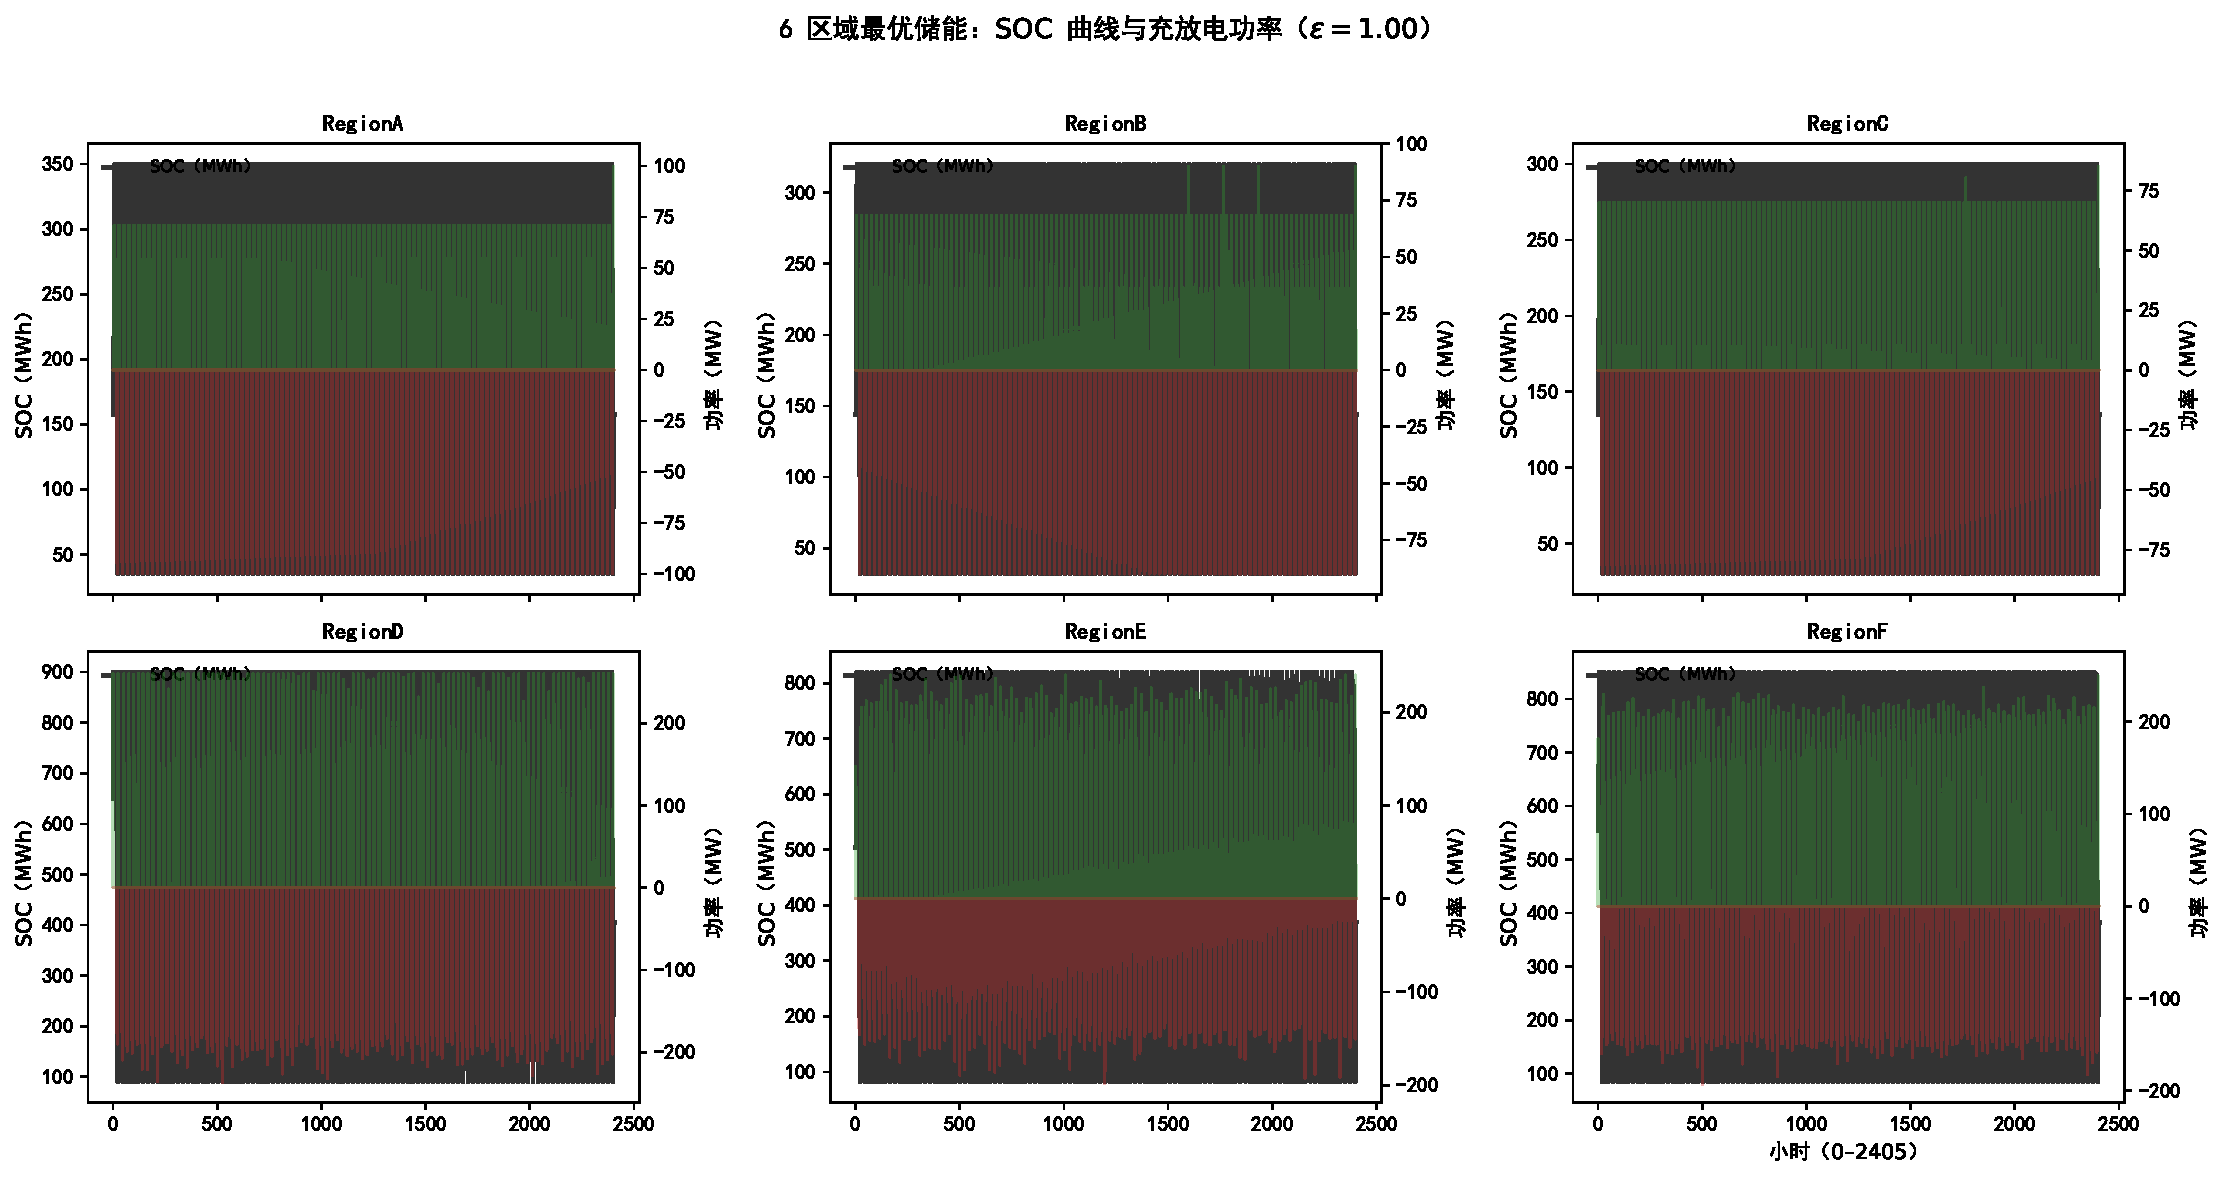
\includegraphics[width=0.95\textwidth]{../../outputs/figures/sub3-soc-charge-discharge-v2.pdf}
\caption{六区域储能 SOC 与充放功率时序（受限消纳 $\varepsilon{=}1.00$）}
\label{fig:soc}
\end{figure}

\section{四指标对比与储能价值}

\begin{table}[h]
\centering
\footnotesize
\begin{tabular}{lcccc}
\toprule
方案 & 成本 (M元) & 碳排 (kt) & 峰值净购电 (MW) & 净购电std (MW) \\
\midrule
\textbf{优化 $\varepsilon{=}1.00$} & \textbf{2213.35} & \textbf{2044.79} & \textbf{550.0} & 686.15 \\
无储能口径 c（诚实下界） & 2387.86 & 2108.00 & 479.0 & 365.43 \\
基准轨迹（参考，不可比） & 1802.34 & 2045.36 & 497.0 & 601.63 \\
基准剔除卖电收入（B3） & 2231.50 & --- & --- & --- \\
\bottomrule
\end{tabular}
\caption{四指标对比（主时域；基准轨迹违反 SOC(2406)$\ge$Initial 且含外送收入，不可直接对比）}
\label{tab:compare}
\end{table}

\textbf{储能价值量级（优化 vs 无储能口径 c）}：成本 $-$174.51 M 元（$-$7.3\%）、
碳排 $-$63.21 kt（$-$3.0\%）、峰值 $+71$ MW（$+14.8\%$，反升）、净购电 std $+87.7\%$（反升）。

\textbf{储能价值归因拆分（阶段 3.1 M10 补实验）}：$-$174.51 M 元 的成本节约
通过"无储能 LP 对照"（D$=$C$^g$$=$C$^r$$=$0、购电时点仍自由优化，受限消纳
$\varepsilon{=}1.00$，聚合成本 2312.71 M 元）拆分为：
\begin{itemize}
  \item $\Delta_2$ \textbf{购电时点自由化价值}：2387.86 $-$ 2312.71 $=$ \textbf{75.15 M 元}（43.1\%）
        ——无储能下优化购电时点即可获得（与时移负荷同效）；
  \item $\Delta_1$ \textbf{储能充放调度价值}：2312.71 $-$ 2213.35 $=$ \textbf{99.36 M 元}（56.9\%）
        ——储能的纯充放调度贡献；
  \item $\Delta_1+\Delta_2 = 174.51$ M 元（精确闭合，$=$ 2387.86 $-$ 2213.35）。
\end{itemize}
结论：$-$7.3\% 中约 57\% 来自储能充放调度、43\% 来自购电时点自由化；
"储能价值"表述限定为\textbf{储能充放调度贡献}，不包含购电时点自由化的收益
（后者在无储能 LP 下同样可达）。

\textbf{成本对照说明（阶段 3.1 修订，原 B3 口径弱化）}：直接对比优化（2213.35）
$>$ 基准（1802.34）会误导——基准含卖电收入（429.16 M 元）且违反终态约束
（不可比）。会计口径下剔除卖电收入后基准成本 $=$ 2231.50 M 元 $>$ 优化
2213.35。\textbf{边界声明}：该对照为\textbf{会计口径}（简单加回卖电收入），
基准的卖电行为与其消纳/购电/储能行为耦合（部分外送透支储能本体能量），并非
"无卖电能力"基准的严格还原；0.8\% 优势在基准构造的任意性面前仅作参考，不作
主结论依据。

\begin{figure}[h]
\centering
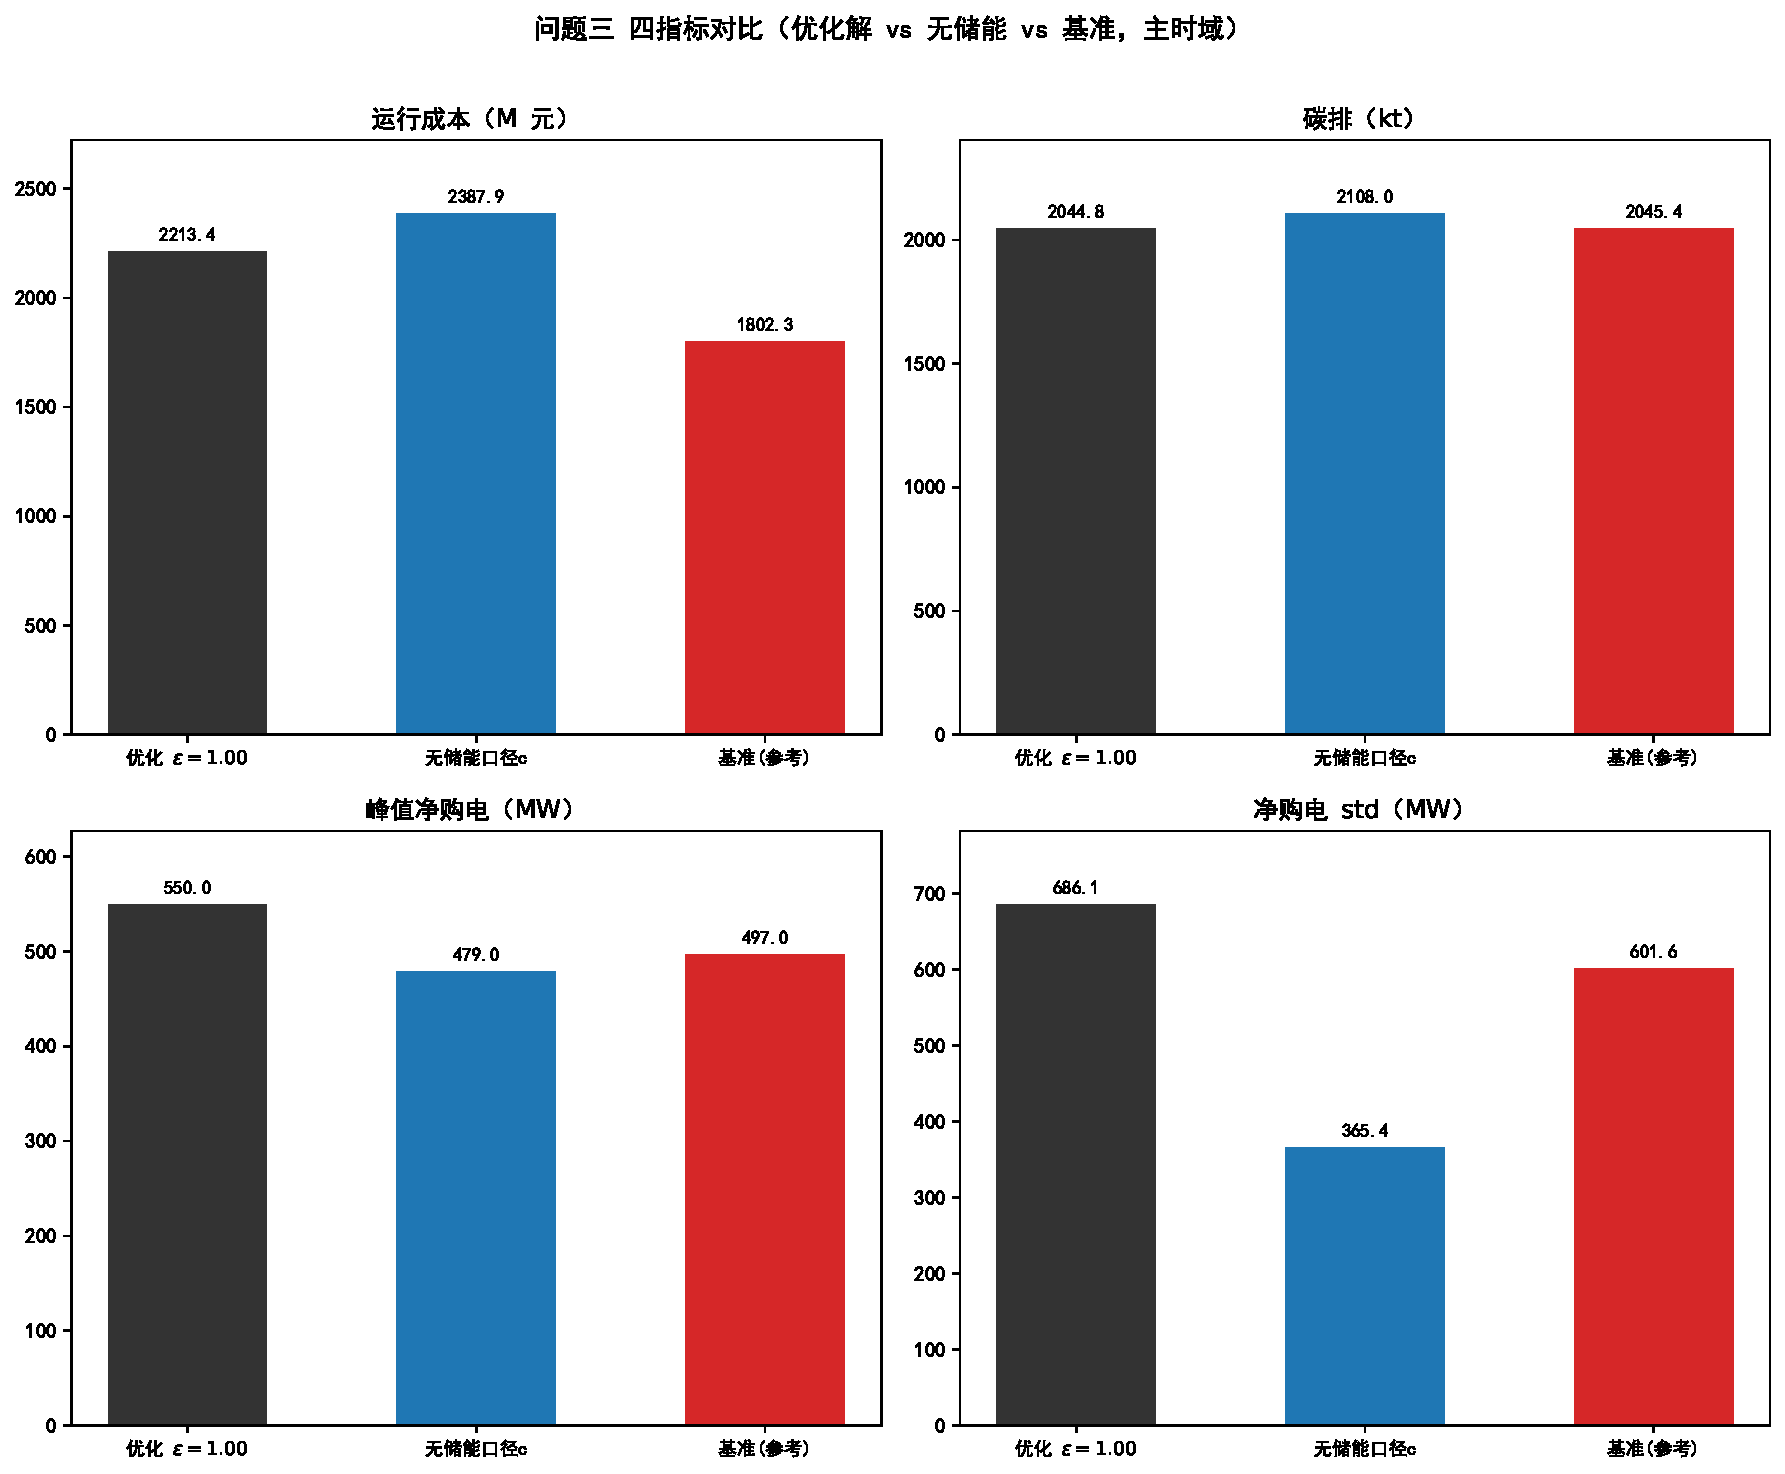
\includegraphics[width=0.95\textwidth]{../../outputs/figures/sub3-four-metrics-v2.pdf}
\caption{四指标三方案对比（成本/碳排/峰值/净购电 std）}
\label{fig:metrics}
\end{figure}

\begin{figure}[h]
\centering
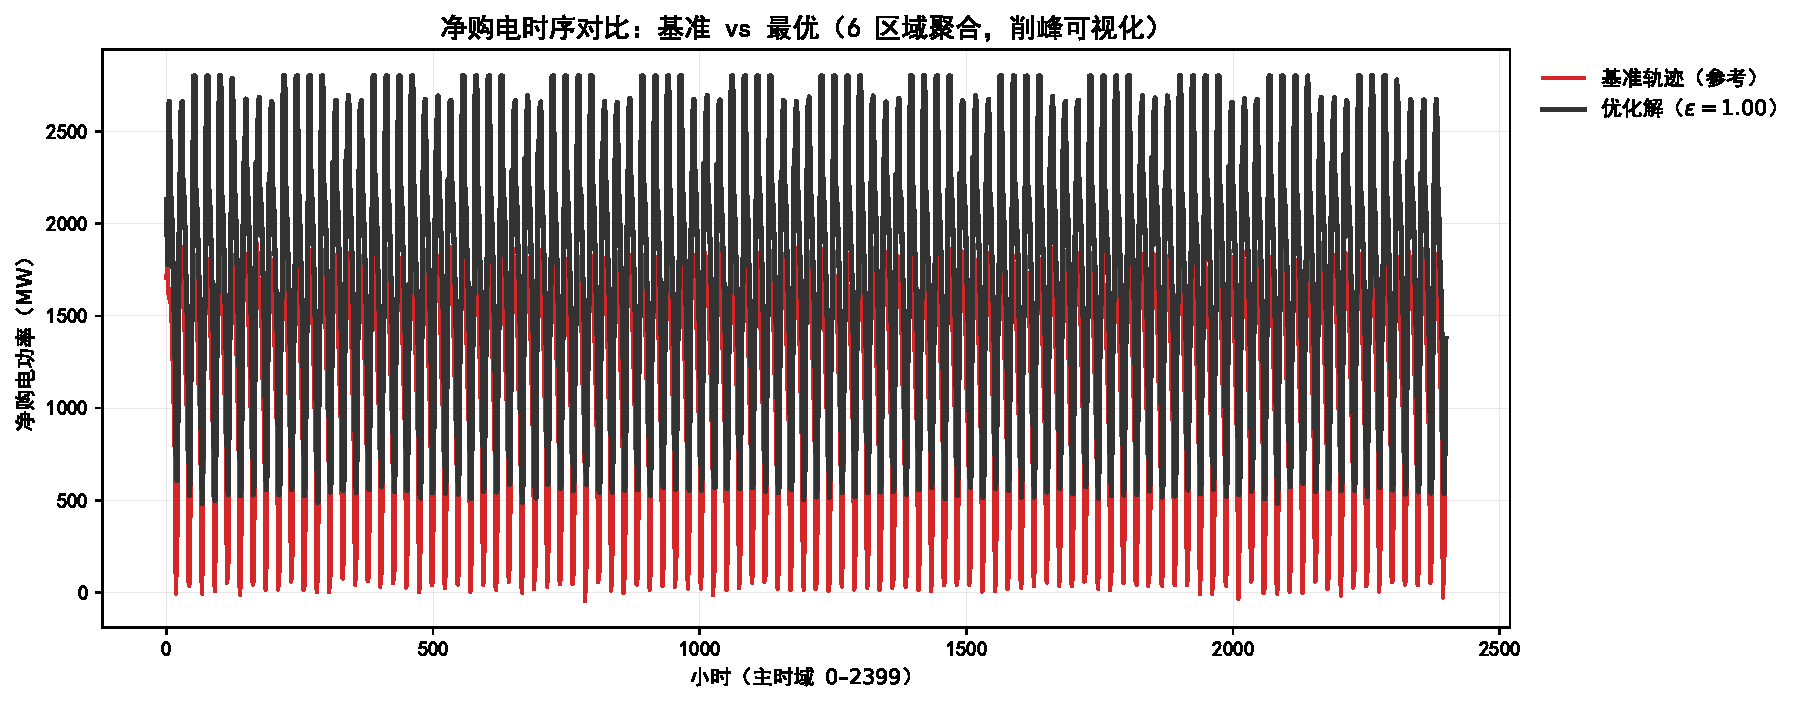
\includegraphics[width=0.95\textwidth]{../../outputs/figures/sub3-net-import-compare-v2.pdf}
\caption{净购电时序对比（基准 vs 最优，削峰/波动形态）}
\label{fig:net}
\end{figure}

\section{关键发现}

\subsection{碳排近乎无压缩空间（给定受限口径下的可行域边界）}

受限消纳把新能源钉在基准水平、负荷固定、储能容量有限，碳排由刚性购电主导。
二分法测定\textbf{给定受限口径下}各区域碳排可行域边界（$\varepsilon_{\min}$，
即碳帽可收紧的极限比例）：

\begin{table}[h]
\centering
\footnotesize
\begin{tabular}{lcccccc}
\toprule
区域 & A & B & C & D & E & F \\
\midrule
碳排下限 $C_{\min}$ (kt) & 577.47 & 516.49 & 480.95 & 254.88 & 80.96 & 108.72 \\
$\varepsilon_{\min}$ & 0.9935 & 0.9938 & 0.9941 & 0.9693 & 0.9574 & 0.9616 \\
较基准压降 & $-0.65\%$ & $-0.62\%$ & $-0.59\%$ & $-3.08\%$ & $-4.26\%$ & $-3.84\%$ \\
\bottomrule
\end{tabular}
\caption{各区域碳排可行域边界 $\varepsilon_{\min}$（$\varepsilon<1.00$ 全部不可行，D4 修订依据）}
\label{tab:emin}
\end{table}

\begin{figure}[h]
\centering
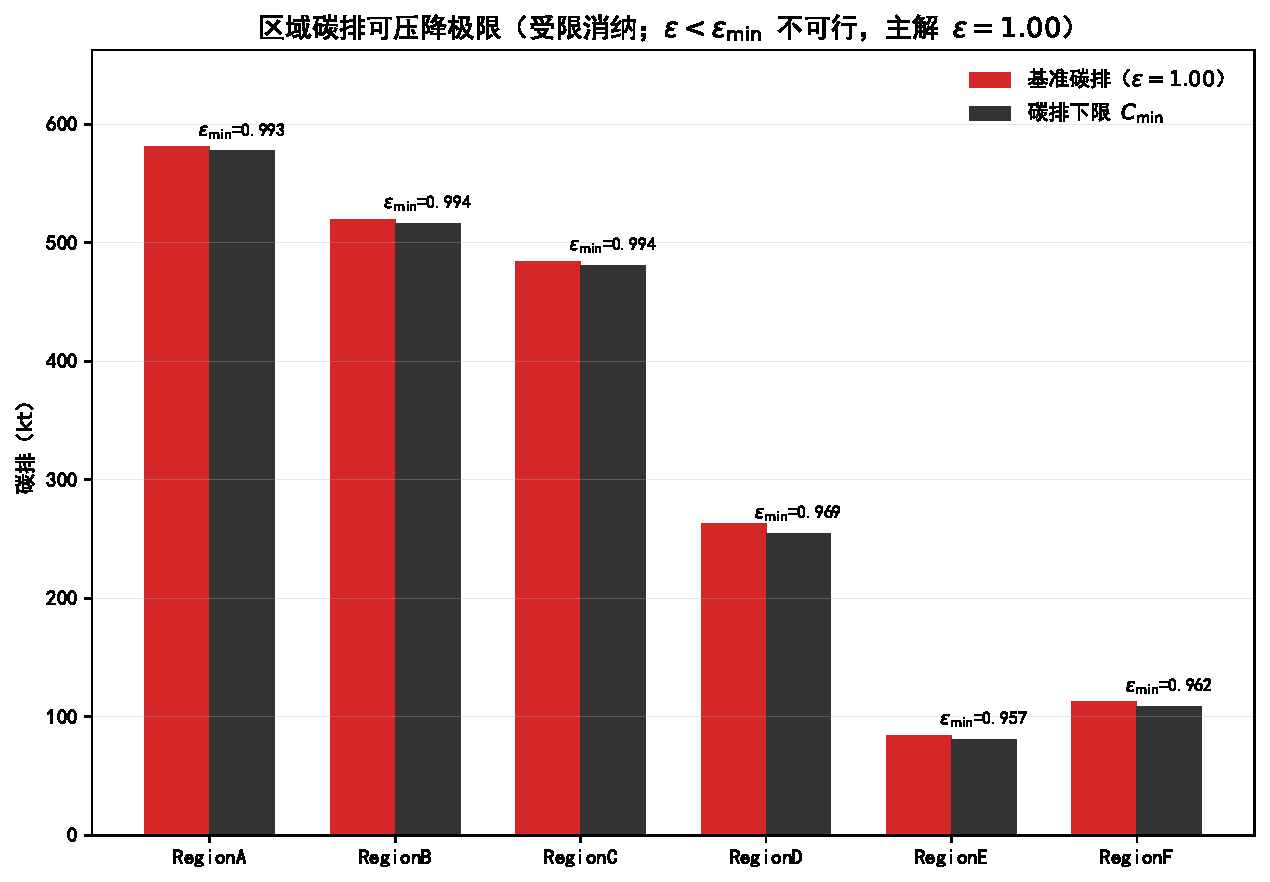
\includegraphics[width=0.85\textwidth]{../../outputs/figures/sub3-carbon-floor-v2.pdf}
\caption{碳排可行域边界可视化（替代 $\varepsilon$ 三档 Pareto——后者不可行）}
\label{fig:floor}
\end{figure}

\subsection{碳--成本--峰值三难（峰值撞顶实证）}

优化解区域峰值净购电撞各区域购电上限（MaxGridImport：A 550/B 520/C 510/D 510/
E 370/F 340 MW），撞顶小时占比 8.5--17.9\%，典型撞顶时段为区域最高碳强度小时
（如 A 区 Hour 51：Price 476.8 元/MWh、CI 0.68 t/MWh）。机理：碳帽 + 受限消纳 +
负荷刚性下，LP 无法回避高碳时段购电，储能削峰空间被碳约束压缩——
\textbf{峰值升高是"碳帽 $\times$ 受限消纳 $\times$ 负荷刚性"耦合的真实代价}，论文按
"碳--成本--峰值三难"正面呈现。

\begin{figure}[h]
\centering
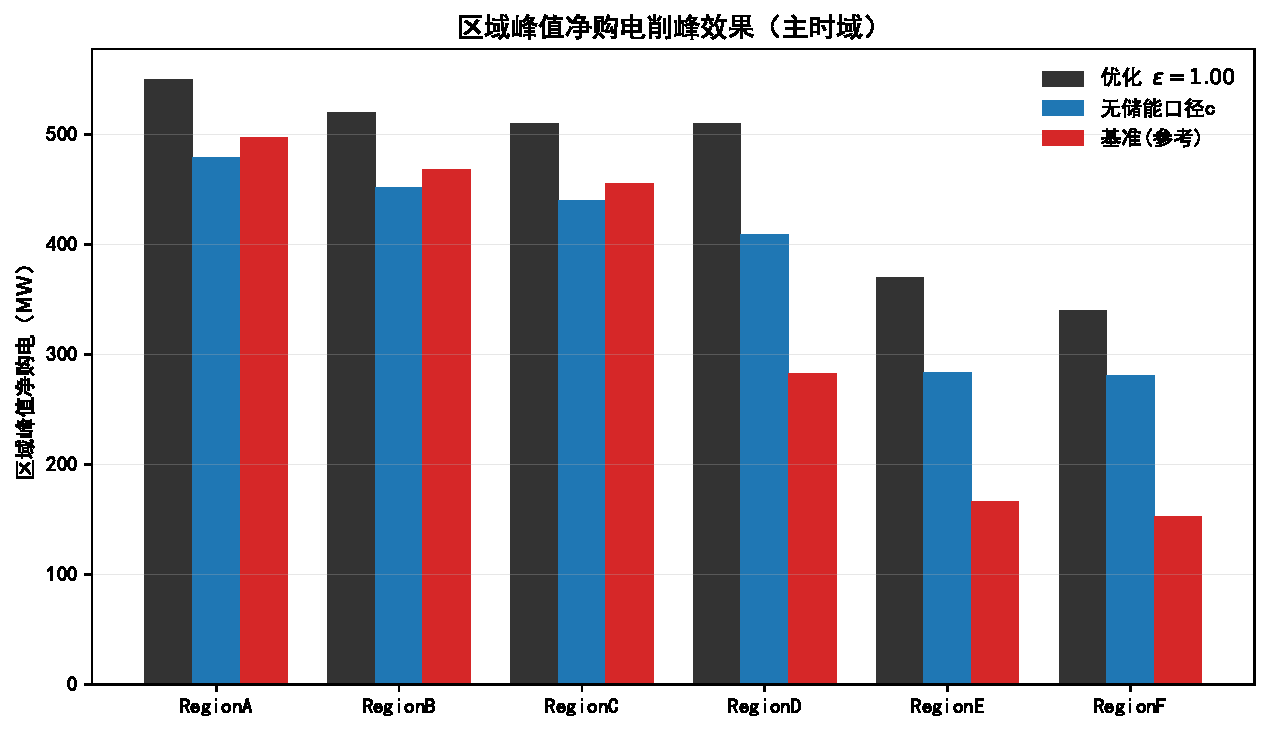
\includegraphics[width=0.85\textwidth]{../../outputs/figures/sub3-peak-shaving-v2.pdf}
\caption{六区域峰值净购电对比（优化撞购电上限）}
\label{fig:peak}
\end{figure}

\subsection{净购电波动反升（诚实呈现 + 口径论证）}

\textbf{负荷波动指标口径（阶段 3.1 补充论证）}：问题三要求分析储能对"负荷波动程度"
的影响。总负荷 $Total\_Load$ 为给定输入（不随储能变化），可被储能改变的是
\textbf{净购电序列}（$G_t-S_t$，与数据列 $NetGridImport$ 同义）；故以净购电 std
为主指标、峰谷差为辅指标，负荷 std 作参照——该口径使"波动度量"成为储能策略的函数，
能反映储能对电网侧波动的真实影响。

\textbf{结果}：成本最小化目标下储能执行峰谷套利（低价时段充电 $\to$ 购电升高、
高价时段放电 $\to$ 购电降低），优化解净购电 std（686.15）\textbf{高于}无储能
（365.43）与基准（601.63），且峰值反升。\textbf{问题三"负荷波动"指标在纯成本
目标下不降反升}——削峰与降本在受限口径下冲突。\textbf{局限说明}：本报告为成本
单目标解，不能回答"储能如何最优地平抑波动"；若以削峰/稳波动为目标需引入多目标
扩展（衔接方案 C/B2 占位，S4 多目标权衡中报告）。

\subsection{卖电消失机制}

D/E/F 的 SellPrice$\le$Price 恒成立（无套利窗口），且受限消纳下新能源优先
直供/充电（R+Cr 用满 cap），故 $S\approx 0$（D/E/F 仅 0--0.8 GWh）。
基准卖电 426--479 GWh 不可复现（其轨迹非最优且违反终态）；利用率双口径
（含/不含外送）在 $S\approx0$ 下趋同（20.83\%/20.84\%）。

\section{拐角解检测}

聚合拐角解比例 0.641（各区域 0.62--0.66），未触发 $>80\%$ "拐角解主导"自动标记，
但比例偏高。解读：高比例主要来自\textbf{结构性绑定}——A/B/C 卖电全时段 $=0$
（S 块 ~1/7 变量在下界）、购电撞顶时段（16--18\%）、SOC 恒在边界（终态 $=$ Initial）。
非病态退化，属约束活性正常分布；论文注明"拐角解集中于结构性约束"。

\section{假设检验回填}

\begin{table}[h]
\centering
\footnotesize
\begin{tabular}{lll}
\toprule
假设 & 检验 & 结果 \\
\midrule
H1 受限消纳锚定基准合理 & 撞顶/绑定小时占比 & $\checkmark$ 撞顶 8.5--17.9\%（购电上限活性） \\
H2 卖电套利成立 & B3 删卖电收入 & $\checkmark$ 无套利（SellPrice$\le$Price）；B3 对照 2231.50$>$2213.35 \\
H3 同刻充放自动排除 & 最优解后验 & $\checkmark$ 六区域同刻充放 $=0$ \\
H4 $\varepsilon$ 档有效 & 全档扫描 & 修订：$\varepsilon<1.00$ 不可行 $\to$ 碳排可行域边界（表 \ref{tab:emin}） \\
H5 终态约束可行 & LP status + SOC & $\checkmark$ status$=0$ 全部；SOC(2406)$\ge$Initial 全合规（恰绑定） \\
H6 结清段碳排 $\approx 0$ & 结清段购电 & $\checkmark$ 结清段无充放、购电极少（基准事实 F8 佐证） \\
\bottomrule
\end{tabular}
\caption{假设检验回填（H1--H6）}
\label{tab:h}
\end{table}

\section{未闭合问题与敏感性}

\begin{enumerate}
  \item 受限消纳假设主导结果：消纳上限为\textbf{消纳能力假设}（基于基准轨迹观测，
        非能力测量，见数据段口径声明）——若真实电网消纳能力不同则成本/碳排量级
        变化；敏感性报告自由消纳口径（购电$\approx0$、成本趋近理想下界）作对照。
  \item 储能价值归因（阶段 3.1 已完成）：$-$7.3\% 已拆分为储能充放调度
        99.36 M 元（57\%）+ 购电时点自由化 75.15 M 元（43\%）（见储能价值归因
        拆分节）；A/B/C 储能近乎空闲（SOC 恒 Initial），储能充放价值集中于
        D/E/F。
  \item 与 S2 $\varepsilon$-约束口径差异：S3 碳排为\textbf{全部设施负荷购电}口径，
        S2 为 AI 任务分量（二者不可相加）；全局碳排以 S3 为主口径、S2 为构成分析；
        两子问题 $\varepsilon$ 均非活跃（S2 未绑定 / S3 不可行），统一叙事
        "$\varepsilon$ 为合规检查、权衡在迁移降碳 vs 储能降本"。
  \item \textbf{口径独立性声明}：问题三"给定任务调度"（官方说明 4）输入为赛题
        给定 Baseline 负荷，与 S2 的优化调度结果\textbf{无数据依赖}——本报告结果
        不与 S2 调度输出耦合。
  \item 储能设备成本（寿命折旧/循环损耗 $\eta_c\eta_d\approx0.86$）未入模，
        论文应注明经济性边界。
\end{enumerate}

\section{结论}

受限消纳主口径下，储能协同优化 LP（$\varepsilon{=}1.00$）给出合规最优解：
聚合成本 2213.35 M 元、碳排 2044.79 kt、峰值净购电 550 MW、净购电 std 686 MW。
较无储能诚实下界：成本 $-7.3\%$、碳排 $-3.0\%$；会计口径剔除卖电收入后基准
（2231.50）略高于优化（2213.35，差 $0.8\%$，仅作参考，见成本对照说明）。
核心结论：\textbf{给定受限口径下碳排已近可行下限（压降 $<$5\%），储能价值集中于
调度优化与终态合规而非消纳提升；成本最小化与削峰/稳波动存在冲突（峰值撞顶、
净购电 std 反升），若需多目标权衡需扩展 $\varepsilon$ 扫描或加权目标}。

\end{document}
